\documentclass[a4paper, 11pt]{report}
\usepackage[british]{babel}
\usepackage{times}
\usepackage{amsmath}
\usepackage{mathtools}
\usepackage{amsfonts}
\usepackage{verbatim}
\usepackage{lmodern}
\usepackage{tikz}
\usepackage[ruled,vlined]{algorithm2e}
\usetikzlibrary{patterns}

\numberwithin{equation}{chapter}

\newtheorem{lemma}{Lemma}[chapter]

\DeclareMathOperator*{\argmax}{arg\,max}
\DeclareMathOperator*{\argmin}{arg\,min}

\DeclareMathOperator*{\KL}{{\rm KL}}
\DeclareMathOperator*{\const}{{\rm const}}

\setlength{\parskip}{1em}

\begin{document}
\SetEndCharOfAlgoLine{}

\title{Bayesian averaging for variational inference applied to genomic data - First Draft}
\author{William van Rooij - EPFL}

\maketitle

\newpage
\tableofcontents
\newpage
\chapter{Introduction}
\section{Situation}
For the past years, data science has been increasingly present in the world. From financial establishments to road management companies, a lot of industry sectors are integrating data science in the way business is done. With the expansion of computer performance, we are able to implement faster computation and can work with more complex models. The volume of available data, hence analysable data, is also growing, which allows more accurate inference.

Often, when trying to find a model for data, we have many more observations than parameters to fit, a \textit{large n, small p} situation. This is the most common type of statistical analysis. Bayesian hierarchical modelling is a strong tool to identify the dependencies across multiple sources of informations, but, the number of parameters may be much larger than the number of observations. This is often the case in genomic research, where the situation is called \textit{small n, large p}. Traditional techniques do not then apply, because of both statistical and computational constraints.

In this report, we will focus on the \textit{small n - large p} situation in the context of genetic association. We will focus on high dimensional Bayesian inference, with its statistical advantages and its computational problem that often dissuades users to adopt this solution in statistical applications.

\section{Motivation}
Current technology allows us to numerically represent the human genome, a whole new set of data is available to study the association between the genome and various diseases or phenotypes.  Some of these newly available data are \textit{genetic variants}, a change at a specific location on  the genome (locus), where the different versions are called \textit{alleles}. We will focus on the most common genetic variant, the \textit{single nucleotide polymorphism} (SNP), a variation in the nucleotide that is present to some appreciable extent in the population. Some combinations of SNPs are inherited together, which yields block-wise dependence structures. We will calculate the association between SNPs and transcript expressions, called \textit{traits}.

The strong correlation structure, observable in Figure \ref{fig:corr}, means that two SNPs in a same correlation block will be hard to differentiate. The goal is two represent the probabilities of association between a SNP and a trait, we should be able to observe the block-wise correlation in our results, the probabilities of association should be high even when the mode is not the real one.

\begin{figure}[h!]
\begin{center}
\includegraphics[width=5in,bb = 0 0 800px 800px]{images/corr_real_SNPs.png}
\caption{\label{fig:corr} Visualisation of the correlation structure in the SNPs. We can clearly see the block-wise correlation structure.}
\end{center}
\end{figure}

We focus on \textit{expression quantitative trait locus} (eQTL) analyses, which study the effects of genetic variants, in our case SNPs, on the expression of transcripts, or genes. The data used for eQTL studies consist generally of several hundred thousands SNPs and thousands of transcripts of expression outcomes. It is, in fact, a \textit{small n, large p, large q} situation, where $p$ is the number of SNPs and $q$ is the number of transcripts of expressions.

Bayesian inference involves many integrals, but these usually need to be approximated. Markov Chain Monte Carlo (MCMC) algorithms are a standard technique for the approximation of integrals and can be fast and accurate when working on reasonably small datasets. When the dataset dimensions grow, however, MCMC algorithms become very time-consuming.

When performing MCMC inference, likelihoods and sometimes gradients need to be calculated at each iteration. The cost of these calculations increases with the number of parameters. Moreover, the more dimensions the problem has, the less accurate the approximations become, requiring more iterations to keep the precision needed. For the algorithm to end, all the parameters need to have converged, which means all parameters need to be checked and stored, which is often impossible when their number is very high.

In our situation, \textit{small n, large p, large q}, the computational cost of using an MCMC algorithm is huge. The time and memory needed to run the algorithm are not acceptable. We have to use an alternative solution, which we choose to be variational inference \cite{varInf}. 

%==========================================
\newpage
\chapter{Model}
Our goal is to estimate the association between a SNP $s$ and a trait $t$. To do so, we let $\boldsymbol{X }= (X_1,\ldots,X_p)$ be the design matrix, representing the SNPs, and $\boldsymbol{y} = (y_1,\ldots,y_q)$ be the response variables, representing the traits. The SNPs have a strong local correlation on the genome.  We consider $\boldsymbol{y}$ as the response matrix and $\boldsymbol{X}$ as the candidate predictors of the linear model, where each response $y_t$ is linearly related with the predictors $\boldsymbol{X}$ and has a residual precision $\boldsymbol{\tau}_t$, i.e.,
\begin{equation*}
\label{eq:model}
\boldsymbol{y}_{n\times q} = \boldsymbol{X}_{n \times p}\;\boldsymbol{\beta}_{p \times q}+\boldsymbol{\epsilon}_{n \times q},\quad\boldsymbol{\epsilon}_t \sim \mathcal{N}(0,\tau_t^{-1}I_n),
\end{equation*}
where $\boldsymbol{\beta}_{st}$ represents the association between SNP $s$ and trait $t$. The parameters $\tau_t$ and $\sigma^{-2}$ have the following prior distributions,
\begin{align*}
\tau_t &\sim \text{Gamma}(\eta_t,\kappa_t),\\
\sigma^{-2} &\sim \text{Gamma}(\lambda,\nu).
\end{align*}

We introduce $\boldsymbol{\gamma}_{p\times q}$, a binary matrix which says which pairs of SNPs and traits are associated. The SNP $s$ and trait $t$ are associated if and only if $\gamma_{st} = 1$. To enforce sparsity in $\boldsymbol{\beta}$, we set a ``spike-and-slab'' prior distribution on $\beta_{st}$, i.e.,
\begin{equation*}
\beta_{st} \mid \gamma_{st},\sigma^2, \tau_t \sim \gamma_{st}\;\mathcal{N}(0,\sigma^2\tau_t^{-1})+(1-\gamma_{st})\;\delta_0,
\end{equation*}
where $\delta_0$ is a Dirac distribution.

We call $\omega_s$ the parameter controlling to the proportion of responses associated with the predictor $X_s$. Then, the prior distribution of $\gamma_{st}$ given $\omega_s$ is:
\begin{equation*}
\gamma_{st} \mid \omega_s \sim  \text{Bernoulli}(\omega_s).
\end{equation*}
We choose $\omega_s$ to follow a Beta distribution,
\begin{equation*}
\omega_s \sim \text{Beta}(a_s, b_s),
\end{equation*}
with parameters $a_s$ and $b_s$ chosen to enforce sparsity. If we define $p^* \ll p$ as the expected number of predictors involved in the model, we want to set $a_s$ and $b_s$ such that the prior probability that $X_s$ is associated with at least one response is equal to $p^*/p$. We fix the mean of the distribution but let the variance be free, the solution still has one degree of freedom so multiple solutions are possible, e.g.,
\begin{equation*}
a_s = 1,\;b_s = q(p-p^*)/p^*.
\end{equation*}



We are interested in estimating the association between the SNPs and the traits, i.e. $\boldsymbol{\beta}$. It is common to estimate the parameters based on the observations $\boldsymbol{y}$, the associated density function is
\begin{align*}
p(\boldsymbol{\beta}\mid\boldsymbol{y})&=\int\dots\int p(\boldsymbol{\beta},\boldsymbol{\gamma},\boldsymbol{\omega},\boldsymbol{\tau},\sigma^{-2}\mid\boldsymbol{y})\;\mathrm{d}\boldsymbol{\gamma}\;\mathrm{d}\boldsymbol{\omega}\;\mathrm{d}\boldsymbol{\tau}\;\mathrm{d}\sigma^{-2},\\
&=\frac{1}{p(\boldsymbol{y})}\int\dots\int p(\boldsymbol{y},\boldsymbol{\beta},\boldsymbol{\gamma},\boldsymbol{\omega},\boldsymbol{\tau},\sigma^{-2})\;\mathrm{d}\boldsymbol{\gamma}\;\mathrm{d}\boldsymbol{\omega}\;\mathrm{d}\boldsymbol{\tau}\;\mathrm{d}\sigma^{-2},\\
\end{align*}
with 
\begin{align*}
p(\boldsymbol{y},\boldsymbol{\beta},\boldsymbol{\gamma},\boldsymbol{\omega},\boldsymbol{\tau},\sigma^{-2}) = &\left\lbrace\prod_{t=1}^qp(\boldsymbol{y}_t \mid \boldsymbol{\beta}_t,\tau_t)\right\rbrace\left\lbrace\prod_{t=1}^q\prod_{s=1}^p p(\beta_{st} \mid \gamma_{st},\tau_t,\sigma^{-2})\right\rbrace\left\lbrace \prod_{t=1}^q\prod_{s=1}^p p(\gamma_{st} \mid \omega_s)\right\rbrace\\
\times &\left\lbrace \prod_{s=1}^p p(\omega_s)\right\rbrace\left\lbrace\prod_{t=1}^q p(\tau_t)\right\rbrace p(\sigma^{-2}),
\end{align*}
where, as mentioned earlier,
\begin{align*}
\boldsymbol{y}_t \mid \boldsymbol{\beta}_t,\tau_t \quad &\sim \quad \mathcal{N}_n\left(\boldsymbol{X}\boldsymbol{\beta}_t,\tau_t^{-1}\boldsymbol{I}_n\right),\\
\beta_{st} \mid \gamma_{st},\tau_t,\sigma^{-2} \quad &\sim \quad \gamma_{st}\mathcal{N}\left(0,\sigma^2\tau_t^{-1}\right)+(1-\gamma_{st})\delta_0,\\
\gamma_{st} \mid \omega_s \quad &\sim \quad \mathrm{Bernoulli}(\omega_s),\\
\omega_s \quad &\sim \quad \mathrm{Beta}(a_s,b_s),\\
\tau_t \quad &\sim \quad \mathrm{Gamma}(\eta_t,\kappa_t),\\
\sigma^{-2} \quad &\sim \quad \mathrm{Gamma}(\lambda, \nu),
\end{align*}
and $\delta_0$ is the Dirac distribution.
% =========================================
\newpage
\chapter{Variational Inference}
When computing the posterior density of parameters $\boldsymbol{\theta}$ according to observed data $\boldsymbol{y}$, variational inference simplifies the computation by approximating the posterior density $p(\boldsymbol{\theta}\mid \boldsymbol{y})$ with a simpler density $q(\boldsymbol{\theta})$. It gives an approximation to the posterior distribution as a result of an optimization problem that minimizes a measure of ``closeness'' as objective function.

If we have observations $\boldsymbol{y}$ and parameters $\boldsymbol{\theta}$, we need to determine the posterior distribution of the parameters conditional on the observations $p(\boldsymbol{\theta} \mid \boldsymbol{y})$. Given a family of densities $\mathcal{D}$ over the parameters, we want to find the distribution $q \in \mathcal{D}$ that minimizes the ``closeness'' measure compared to $p(\boldsymbol{\theta} \mid \boldsymbol{y})$.

Variational inference minimizes the Kullback--Leibler divergence as a ``closeness'' measure. Introduced in 1951 by Kullback and Leibler\cite{kl51}, this is the most common divergence measure used in statistics and machine learning:
\begin{equation*}
\KL(q\parallel p) := \int q(\boldsymbol{\theta})\log \left(\frac{q(\boldsymbol{\theta})}{p(\boldsymbol{\theta} \mid \boldsymbol{y})}\right) \mathrm{d}\boldsymbol{\theta}.
\end{equation*} 
It is described as a "directed divergence" as it is asymmetric, i.e., $\KL(p\parallel q) \neq \KL(q \parallel p)$.

Determining the family $\mathcal{D}$ can be difficult, as we need the family to be simple enough to be optimized efficiently, but flexible enough for the approximation $q \in \mathcal{D}$ to be close to $p(\boldsymbol{\theta} \mid \boldsymbol{y})$ with respect to the Kullback--Leibler divergence. The approximation will then be
\begin{equation*}
q^*(\boldsymbol{\theta} ) = \argmin_{q(\boldsymbol{\theta}) \in \mathcal{D}} \KL\left[ q(\boldsymbol{\theta}) \parallel p(\boldsymbol{\theta} \mid \boldsymbol{y})\right].
\end{equation*}

Minimizing the Kullback--Leibler divergence can be complicated depending on the density $p$ that we want to approximate and the density family $\mathcal{D}$ that we want $q$ to be part of. We can decompose the Kullback--Leibler divergence as
\begin{align*}
\KL\left[q(\boldsymbol{\theta})||p(\boldsymbol{\theta}\mid \boldsymbol{y})\right] &= \mathbb{E}\left[\log q(\boldsymbol{\theta})\right] - \mathbb{E}\left[\log p(\boldsymbol{\theta}\mid \boldsymbol{y})\right]\\
&= \mathbb{E}\left[\log q(\boldsymbol{\theta})\right] - \mathbb{E}\left[\log p(\boldsymbol{y},\boldsymbol{\theta})\right] + \log p(\boldsymbol{y}).
\end{align*}
We introduce the evidence lower bound:
\begin{equation*}
\mathcal{L}(q) = \mathbb{E}\left[\log p(\boldsymbol{\theta},\boldsymbol{y})\right] - \mathbb{E}\left[\log q(\boldsymbol{\theta})\right]
=\int q(\boldsymbol{\theta})\log\frac{p(\boldsymbol{y},\boldsymbol{\theta})}{q(\boldsymbol{\theta})}\mathrm{d}\boldsymbol{\theta}.
\end{equation*}
When decomposing the Kullback--Leibler divergence, we obtain
\begin{equation*}
\KL(q\parallel p) = \log(p) - \mathcal{L}(q).
\end{equation*}
This means that the Kullback--Leibler divergence is the difference between the marginal log-likelihood with no effect on the optimization and a function $\mathcal{L}(q)$. Hence, minimizing the Kullback--Leibler divergence is the same as maximizing $\mathcal{L}(q)$. The difference lies in the complexity of the problems, minimizing the Kullback--Leibler divergence is not tractable, but maximizing $\mathcal{L}(q)$ admits a closed form when the family of densities $\mathcal{D}$ is well chosen. In such a case, we prefer to use $\mathcal{L}(q)$ as an objective function.

Jensen's inequality provides another way to see that $\mathcal{L}(q)$ is a lower bound for the marginal log-likelihood, which is why we call it the evidence lower bound, or variational lower bound,
\begin{align*}
\log p(\boldsymbol{y}) &= \log \int p(\boldsymbol{y}, \boldsymbol{\theta}) \mathrm{d}\boldsymbol{\theta},\\
&= \log \int \frac{p(\boldsymbol{y}, \boldsymbol{\theta})}{q(\boldsymbol{\theta})}q(\boldsymbol{\theta})\mathrm{d}\boldsymbol{\theta}
,\\
&\geq \int q(\boldsymbol{\theta}) \log \left\lbrace \frac{p(\boldsymbol{y}, \boldsymbol{\theta})}{q(\boldsymbol{\theta})} \right\rbrace \mathrm{d}\boldsymbol{\theta},\\
&= \mathcal{L}(q).
\end{align*}
Hence, $\log p(\boldsymbol{y}) \geq \mathcal{L}(q)$.

\section{Mean-field approximation}
The complexity of the optimization problem is directly bound to the complexity of the family of densities $\mathcal{D}$ to which $q(\boldsymbol{\theta})$ belongs. We introduce the mean-field variational family, where the parameters are mutually independent.

Let $\left\lbrace \theta_j\right\rbrace_{j=1}^J$ be a partition of $\boldsymbol{\theta}$, $q \in \mathcal{D}$ and $\mathcal{D}$ a mean-field variational family, then,
\begin{equation*}
q(\boldsymbol{\theta}) = \prod_{j=1}^J q_j(\theta_j).
\end{equation*}
We determine the variational factors $q_j(\theta_j)$ by maximizing $\mathcal{L}(q_j)$. Hence, the variational family does not directly represent the observed data, they are both linked through the optimization of the evidence lower bound.

Concretely, we assume the independence of most of the parameters,
\begin{equation*}
q(\boldsymbol{\theta}) =\left\lbrace\prod_{s=1}^p \prod_{t=1}^q q(\beta_{st}, \gamma_{st})\right\rbrace \left\lbrace\prod_{s=1}^p  q(\omega_s)\right\rbrace \left\lbrace\prod_{t=1}^q q(\tau_t)\right\rbrace q(\sigma^{-2}).
\end{equation*}


\begin{figure}[h!]
\centering
\begin{tikzpicture}
\draw[thick, ->] (0,-2) -- (0,2);
\draw[thick, ->] (-2,0) -- (2,0);
\fill[pattern=north west lines,opacity=.6,draw] (0,0) circle (1cm);
\draw[rotate=-45] (0,0) ellipse (0.65cm and 2cm);
\node (p) at (2,1.7) {Real posterior};
\node (q) at (2.7,-0.9) {Mean-field approximation};
\node (x1) at (-0.3,2) {$x_1$};
\node (x2) at (2,-0.3) {$x_2$};
\end{tikzpicture}
\caption{\label{fig:mean_field}To visualise the mean-field approximation, we consider a two dimensional Gaussian distribution, represented in clear in Figure \ref{fig:mean_field}. The mean-field approximation of the posterior distribution is represented by the barred circle. We see that the mean of the approximation is the same as the real mean, but the covariance does not match the covariance of the real posterior.}
\end{figure}

We have transformed, using the evidence lower bound and the mean-field approximation our problem into a optimization problem. We now need a way to solve this problem. In the following section, we describe the coordinate ascent algorithm.
% =========================================
\section{Coordinate ascent algorithm}
Coordinate ascent mean-field variational inference  is one of commonly used to solve this optimization problem. The algorithm iterates on the parameters of the mean-field approximation, optimizing them one at the time. It yields a local optimum for the evidence lower bound. The algorithm is based on the following result:
\begin{lemma}

If we fix $q_l(\theta_l)$, $l\neq j$, then the optimal $q^*_j(\theta_j)$ satisfies:
\begin{equation*}
q^*_j(\theta_j) \propto \exp\left\lbrace\mathbb{E}_{-j}\left[\log p(\theta_j \mid \boldsymbol{\theta}_{-j}, \boldsymbol{y})\right]\right\rbrace.
\end{equation*}
Where $\mathbb{E}_{-j}$ denotes the expectation with respect to all $\theta_l$, $l \neq j$.
\end{lemma}

Based on this result, the algorithm updates one parameter $\theta_j$ at a time while the others stay fixed. The algorithm stops when $\mathcal{L}(q)$ increases by less than a pre-determined threshold $\varepsilon$.

\begin{algorithm}
\SetKwData{ELBO}{$\mathcal{L}(q)$}\SetKwData{OLDELBO}{$\mathcal{L}^{\text{old}}(q)$}
\SetKwFunction{Union}{Union}\SetKwFunction{FindCompress}{FindCompress}
\SetKwInOut{Input}{input}\SetKwInOut{Output}{output}\SetKwInOut{Init}{initialize}
\SetKw{Set}{set}
\Input{$p(\boldsymbol{y},\boldsymbol{\theta})$, dataset $y$ tolerance $\varepsilon$}
\BlankLine
\Output{$q(\boldsymbol{\theta}) = \prod_{j=1}^J q_j(\theta_j)$}
\BlankLine
\Init{$q_j(\theta_j)$}
\BlankLine
\Repeat{$|$\OLDELBO$-\mathcal{L}(q)| < \varepsilon $}{
\For{$j\in \left\lbrace 1, \ldots, J \right\rbrace $}{
\Set{$q_j(\theta_j) \propto \exp\left\lbrace\mathbb{E}_{-j}\left[\log p(\theta_j \mid \boldsymbol{\theta}_{-j}, \boldsymbol{y})\right]\right\rbrace$}}
\BlankLine
\OLDELBO$\leftarrow$\ELBO\\
\ELBO$\leftarrow\mathbb{E}\left[\log p(\boldsymbol{\theta}, \boldsymbol{y})\right]-\mathbb{E}\left[\log q(\boldsymbol{\theta})\right]$
\BlankLine
}
\Return{$q(\boldsymbol{\theta})$}
\caption{Coordinate ascent variational inference \label{alg:CAVI}}
\end{algorithm}
At every iteration, $\mathcal{L}(q)$ is guaranteed to increase. The algorithm yields a local optimum depending on the initialization of the $q_j(\theta_j)$, $j=1,\ldots,J$. Having different initializations could yield different optima that correspond to different models.

In our case, the posterior distributions of our model's parameters are:
\begin{align*}
\beta_{st} \mid \gamma_{st} = 1, \boldsymbol{y} &\sim \mathcal{N}\left(\mu_{\beta, st},\sigma^2_{\beta, st}\right),\\
\beta_{st} \mid \gamma_{st} = 0, \boldsymbol{y} &\sim \delta_0,\\
\gamma_{st} \mid \boldsymbol{y} &\sim \text{Bernoulli}(\gamma_{st}^{(1)}),\\
\omega_s\mid\boldsymbol{y} &\sim \text{Beta}(a_s^*,b_s^*),\\
\tau_t\mid \boldsymbol{y} &\sim \text{Gamma}(\eta^*_t, \kappa^*_t),\\
\sigma^{-2} \mid \boldsymbol{y} &\sim \text{Gamma}(\lambda^*, \nu^*).
\end{align*}

\newpage
\chapter{Multimodality}

Bayesian model averaging is a strategy to account for multiple competing models in an inference problem. It consists of weighting the different models in a weighted average with the probability that the data corresponds to each model. The more the model corresponds to the observed data, the more it will stand out in the result.

Assume that the data $\boldsymbol{y}$ correspond to multiple models $M_k$, $k= 1,\ldots,K$, and $\Delta$ is the quantity of interest. We have the posterior distribution:
\begin{equation}
p(\Delta \mid \boldsymbol{y}) = \sum_{k=1}^K p(\Delta \mid M_k,\boldsymbol{y}) \; p(M_k \mid \boldsymbol{y}).
\label{eq:post_dist}
\end{equation}
This corresponds to a weighted average of the posterior distribution under each of the considered models with weights corresponding to the posterior models probabilities.

Instead of $p(\Delta \mid \boldsymbol{y})$ in Equation \ref{eq:post_dist}, we might be interested in approximating:
\begin{equation*}
\mathbb{E}\left[\Delta \mid \boldsymbol{y}\right] = \sum_{k=1}^K\mathbb{E}\left[\Delta \mid M_k, \boldsymbol{y}\right]\;p(M_k \mid \boldsymbol{y}).
\end{equation*}

The posterior probability for model $M_k$ is given by:
\begin{equation}
p(M_k \mid \boldsymbol{y}) = \frac{p(\boldsymbol{y} \mid M_k)\; p(M_k)}{\sum_{j=1}^K p(\boldsymbol{y} \mid M_j)\; p(M_j)},
\label{eq:post_prob}
\end{equation}
where $p(\boldsymbol{y} \mid M_k)$ is the likelihood of model $M_k$, and $p(M_k)$ is the prior probabilities of the model $M_k$. It can, for example, depend on the complexity of the model, to favour the simpler models, or, if we consider the models to be equiprobable, it would be equal to $p(M_k) = 1/K$, $k = 1,\ldots,K$.  

We know that the evidence lower bound and the Kullback--Leibler divergence are related and that minimizing the Kullback--Leibler divergence is equivalent to maximizing the evidence lower bound, and that they verify: 
\begin{equation*}
\KL(q\parallel p) = \log p (\boldsymbol{y}) - \mathcal{L}(q).
\end{equation*}
Since we minimized the Kullback--Leibler divergence, we can use $\mathcal{L}(q)$ as an approximation for $\log p(\boldsymbol{y})$ in Equation \ref{eq:post_prob}.

Our quantity of interest is $\gamma_{st}$, i.e. we want to know if the SNP $s$ and the trait $t$ are associated. Using Algorithm \ref{algo:CAVI}, we initialise the distributions $q_j(\theta_j)$ with different starting points, and consider the optimums yielded by the algorithm.

We can consider each optimum to be a model representing the data, and we can apply a form of Bayesian model averaging to combine them all using the method we described here above. We approximate $\log p(\boldsymbol{y})$ by $\mathcal{L}(q)$ in Equation \ref{eq:post_prob}, and obtain an approximation for $\mathbb{E}\left[\gamma_{st}\mid \boldsymbol{y}\right]$ considering all the models we have obtained in the algorithm.

As we are dealing with strongly correlated structures, some modes will be strongly plausible even if they are not the real mode. This incertitude should be visible when observing the resulting approximations for $\mathbb{E}\left[\gamma_st\mid \boldsymbol{y}\right]$. Indeed, we should see the real mode standing out, but we should have some other modes visible as well, more or less visible according to their plausibility.
\newpage
\section{Simulated Annealing}
To identify data dependence structures, instead of altering the model, we can change the inference strategy. When dealing with highly correlated data, our coordinate ascent algorithm often gets stuck in local modes. We use a simulated annealing procedure to augment our method and improve the modes exploration.

We start with the same strategy as earlier, i.e. minimizing the reverse Kullback--Leibler divergence,
\begin{equation*}
\KL(q \parallel q) = -\int q(\boldsymbol{\theta}) \log\left\lbrace\frac{p(\boldsymbol{\theta}\mid\boldsymbol{y})}{q(\boldsymbol{\theta})}\right\rbrace \mathrm{d}\boldsymbol{\theta}.
\end{equation*}
we end up with the lower bound as objective function,
\begin{equation*}
\mathcal{L}(q) = \mathbb{E}_q\left[ \log p(\boldsymbol{y}, \boldsymbol{\theta})\right] - \mathbb{E}_q\left[\log q(\boldsymbol{\theta})\right],
\end{equation*}
which is composed of the expected log joint distribution, which motivates the approximation to take more mass where the variables explain more the data, and the entropy, that encourages the dispersion of the approximation. 

The idea of simulated annealing is to introduce a temperature $T$ that yields a series of heated distributions,
\begin{equation*}
p_T(\boldsymbol{y},\boldsymbol{\theta}) \propto p(\boldsymbol{y},\boldsymbol{\theta})^{1/T},
\end{equation*}
and influences the differences of the modes. The temperature starts high, smoothing the density of interest, and gets lower along the process until it reaches the original density. The high temperatures yield an easier search for the global optimum. The temperature multiplies the entropy term, allowing for more disparate approximations to be considered,
\begin{equation}
\mathcal{L}_T(q) = \int q_T(\boldsymbol{\theta}) \log p(\boldsymbol{y},\boldsymbol{\theta})\mathrm{d}\boldsymbol{\theta} - T \int q_T(\boldsymbol{\theta}) \log q_T(\boldsymbol{\theta}) \mathrm{d}\boldsymbol{\theta},\; T\geq 1,
\label{eq:ann_elbo}
\end{equation}
where $q_T$ is the heated variational distribution, it applies a penalty on the log joint distribution when the temperature $T > 1$, and relaxes the penalty as $T$ goes down until $T = 1$, where the penalty becomes null.

With the same process we used without the annealing, we can write (\ref{eq:ann_elbo}) with respect to $\theta_j$ as
\begin{equation*}
\mathcal{L}_T(q) = \mathbb{E}_j\left[\mathbb{E}_{-j}\left\lbrace \log p(\boldsymbol{y},\boldsymbol{\theta})\right\rbrace - T \log q_T(\theta_j)\right]+ \const,
\end{equation*}
that can be written as
\begin{equation*}
\mathcal{L}_T(q) = T\mathbb{E}_j\left[\log\left\lbrace\frac{p_{T, -j}(\boldsymbol{y}, \theta_j)}{q_T(\theta_j)}\right\rbrace\right] + \const,	
\end{equation*}
where $p_{T, -j}(\boldsymbol{y},\theta_j) \propto \exp\left\lbrace T^{-1}\mathbb{E}_{-j}\left[\log p(\boldsymbol{y},\boldsymbol{\theta})\right]\right\rbrace$, $\mathbb{E}_j$ is the expected value with respect to $q_T(\theta_j)$, $\mathbb{E}_{-j}$ is the expected value with respect to every $ q_T(\theta_k)$ where $k \neq j$, and $\const$ is independent of $v_j$.

$\mathcal{L}_T(q)$ is maximal when $q_T(\theta_j) = p_{T,-j}(\boldsymbol{y},\theta_j)$, which is equivalent to when
\begin{equation*}
\log q_T(\theta_j) = T^{-1} \mathbb{E}_{-j}\left[\log p(\boldsymbol{y}, \boldsymbol{\theta})\right] + \const\text{,}\quad j=1,\dots,J.
\end{equation*}

We have a choice to make for the temperature schedule to consider, we have chosen to take a geometric spacing,
\begin{equation*}
T_l = (1 + \Delta)^{l-1},\quad \Delta = T_L^{1/(L-1)}-1,
\end{equation*}
where $l = 1,\dots,L$ and $T_L$ is the hottest temperature. $T_l$ is the temperature used at step $l$ and $L$ is the number of steps necessary to lower the temperature to the initial temperature $T = 1$, where the initial algorithm is ran until convergence.

To cope with strongly correlated structures and represent the incertitude of the modes, we use simulated annealing combined with our weighted average and retrieve a combination of different models yielded from different initialisations. However, two different initialisations that gave different modes could give the same mode when using simulated annealing as the density function is ``smoothed'' by the temperature. The number of different modes considered in the weighted average will hence be less than when not performing the simulated annealing step before hand.

% =========================================
\newpage
\chapter{Simulations}
In her R-package \texttt{locus}, H. Ruffieux has implemented a function \texttt{locus} that estimates the probabilities of association between a SNP and a trait. We will use this function to build our own method and also to have a comparison. If our method would not perform better than this implementation, it because irrelevant.

Our method is basically calling multiple times that \texttt{locus} function and combine all the results in an weighted average. For each call, we initialized the parameters differently, and hoped to obtain different optimums. We will call this method ``multiple locus'', the single call method will be ``single locus'' and when augmented with simulated annealing, we will just add ``annealing'' before the name.

We have drawn at random the initial parameters for the optimal approximations $q^*(\boldsymbol{\theta})$. We have used H. Ruffieux's function \texttt{locus} to calculate the probabilities of association between the SNPs and the traits, as well as the evidence lower bound for each initialisation. Then we used the evidence lower bounds as weights in our variant of Bayesian model averaging to combine the results of each initialisation.

We first tested our method on generated data, to be able to compare the results calculated with the truth. We have used H. Ruffieux's R-package \texttt{echoseq} to generate block wise strongly autocorrelated SNPs and traits, as well as their associations. We have generated $300$ observations of $500$ SNPs, with autocorrelations between $0.95$ and $0.99$, by blocks of $10$ SNPs. As we want to visualise the probabilities of association, we generated just one trait. We did $100$ random initialisations of the parameters.

We wanted to compare four methods, single locus, multiple locus and their simulated annealing augmented counterparts. We chose four different situations that we thought would be interesting to compare. Two of the settings were constituted of $15$ associated SNPs, whereas the two other had $50$ associated SNPs. We also had a pair of settings where the proportion of the response variance that could be explained by the SNPs could be up to $50\%$ and, for another pair, up to $80\%$.

\begin{figure}[h!]
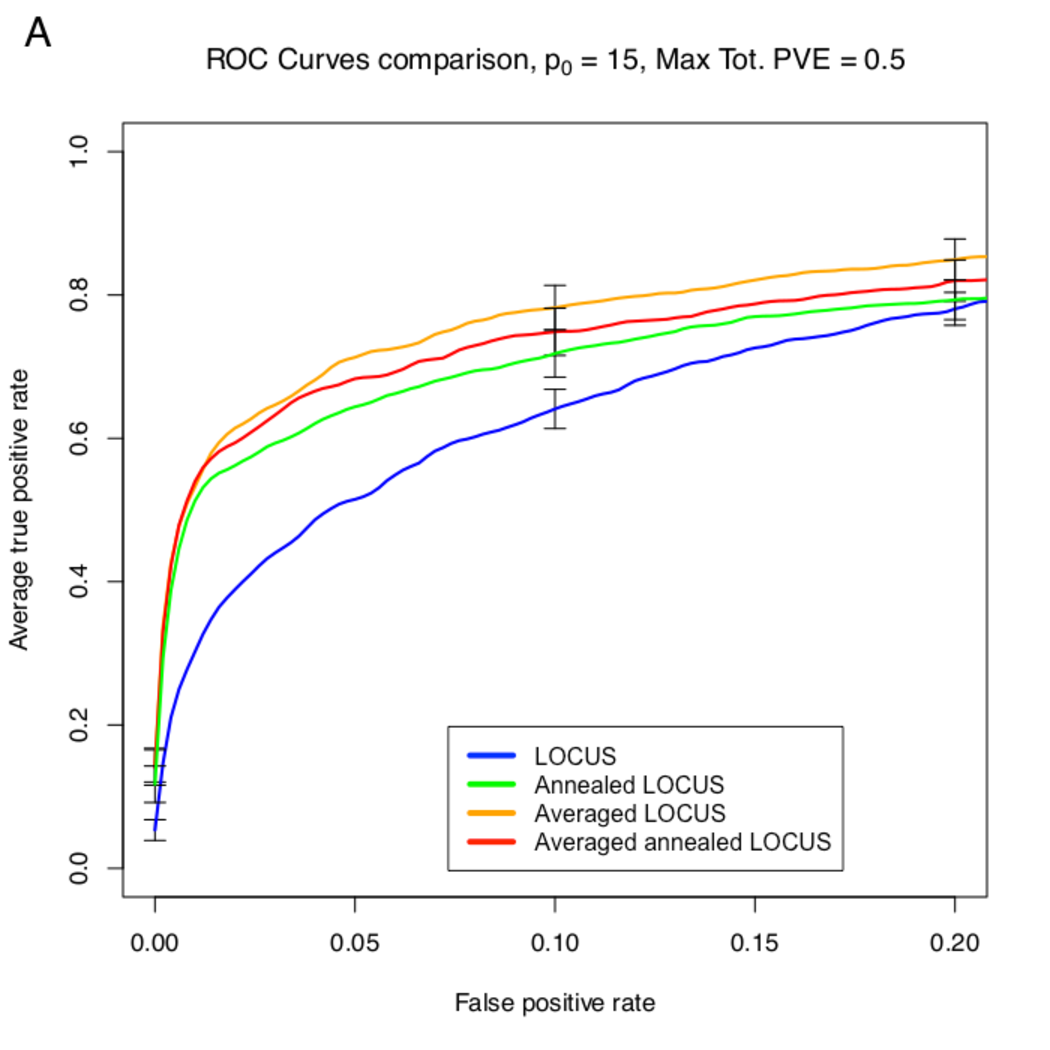
\includegraphics[width=2.6in, bb=0 0 500 500]{images/ROC_Comp_p0_15_var_0_5.pdf}
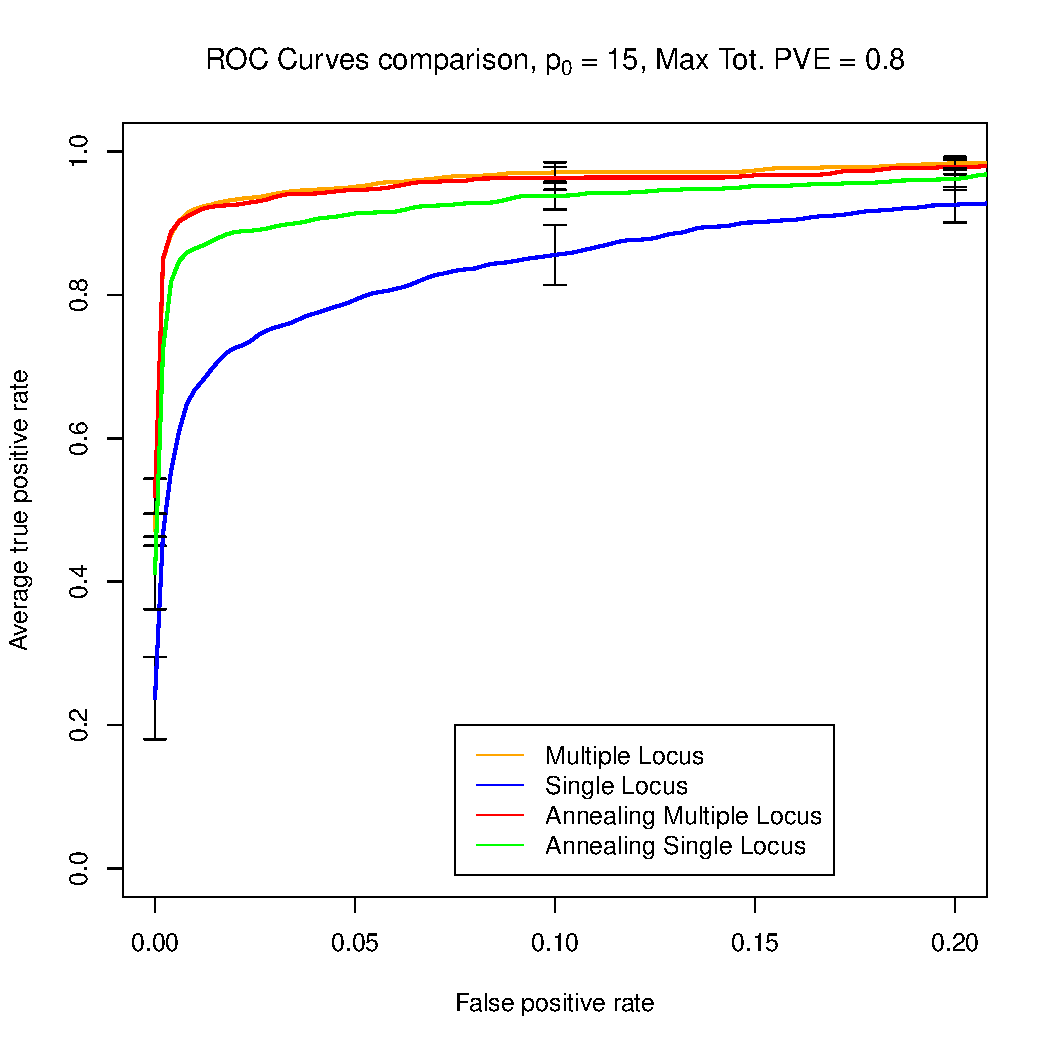
\includegraphics[width=2.6in, bb=0 0 500 500]{images/ROC_Comp_p0_15_var_0_8.pdf}
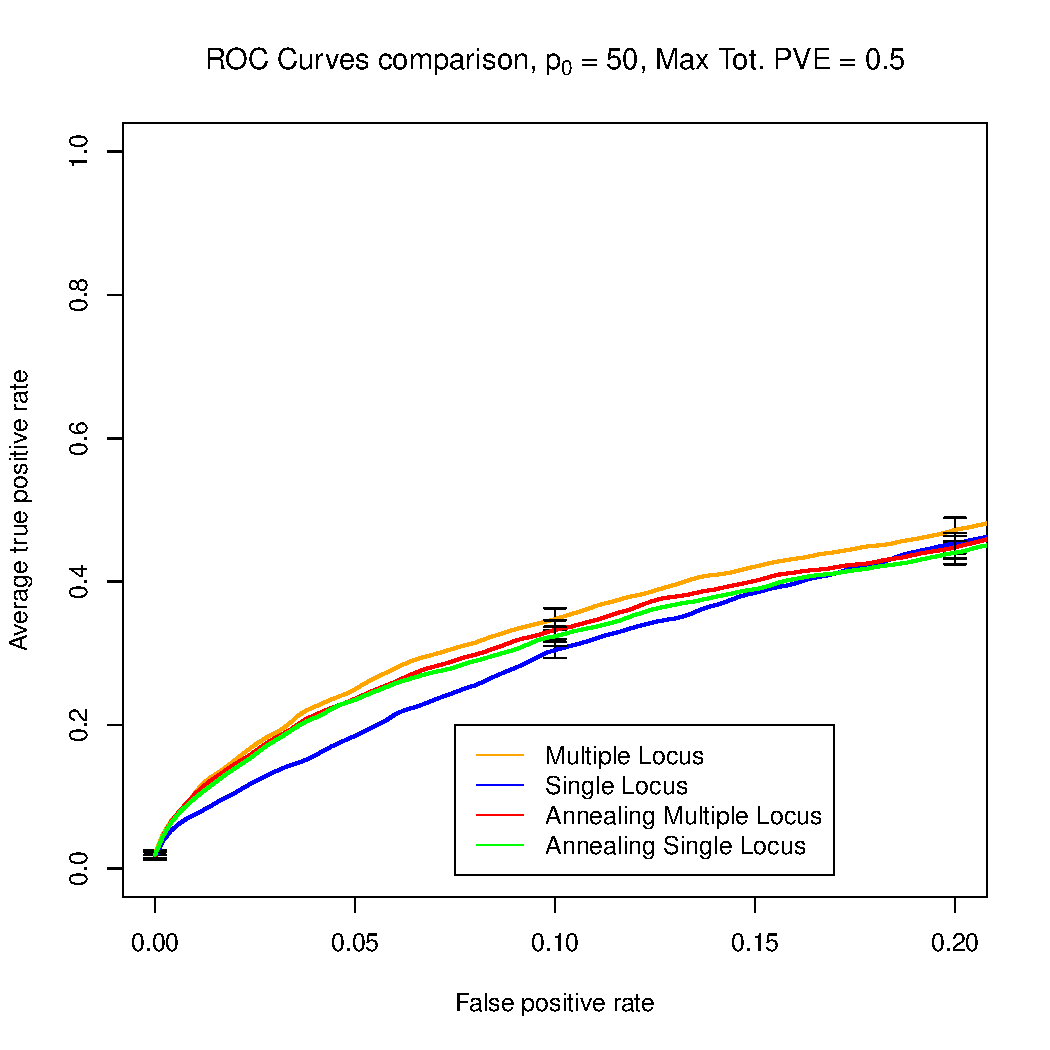
\includegraphics[width=2.6in, bb=0 0 500 500]{images/ROC_Comp_p0_50_var_0_5.pdf}
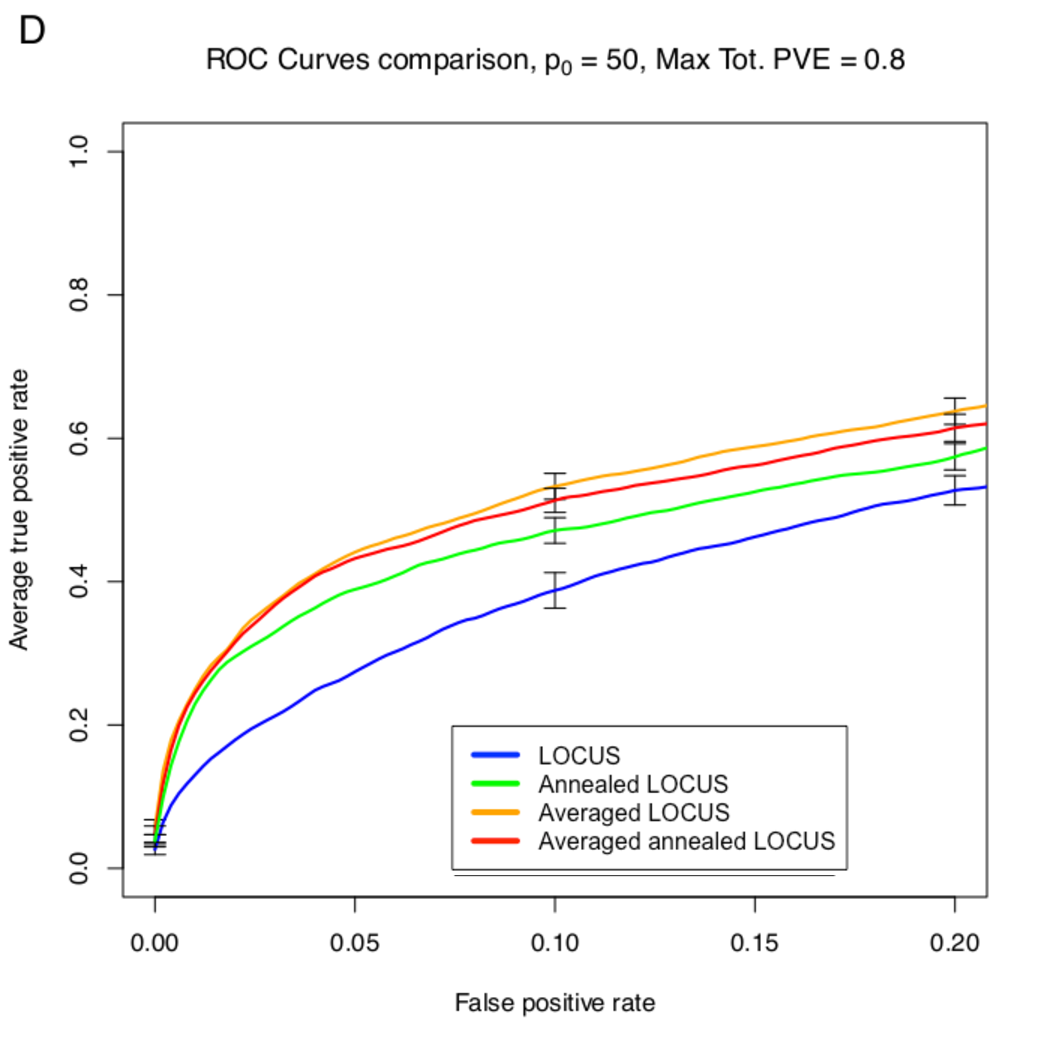
\includegraphics[width=2.6in, bb=0 0 500 500]{images/ROC_Comp_p0_50_var_0_8.pdf}
\caption{\label{fig:ROCComp}Comparison of ROC curves between multiple and single locus, and the same two methods augmented with a simulated annealing step, colored orange, blue, red, and green respectively. Top row: $p_0 = 15$, Left column: Max tot. PVE$ = 0.5$,
Bottom row: $p_0 = 50$, Right column: Max tot. PVE$ = 0.8$}
\end{figure}
In Figure \ref{fig:ROCComp} are represented the ROC curves of the four methods we wanted to compare, for each of the four settings we mentioned earlier. We have truncated the ROC curves as we are interested only in the accuracy of the methods for a small error rate. 

Firstly, we will compare the single locus and the multiple locus methods. We can clearly see in Figure \ref{fig:ROCComp} that the multiple locus is much mote accurate than the single locus. The multiple locus considers many different modes, in our case $100$, and attributes to each mode a weight associated to the likelihood of the data being obtained from said mode.

It should be noted that for our method, paralleled computation is possible, which can drastically diminish the time needed to compute it. Even if the method has to wait until the last iteration to converge, we would still be quicker than calculating the iterations one after the other.

\begin{center}
\begin{figure}[h]
\includegraphics[width=2.7in, bb= 0 0 175 175]{images/s_locus.png}
\includegraphics[width=2.7in, bb= 0 0 175 175]{images/m_locus.png}
\caption{\label{fig:simple_locus}Probabilities of association of the $50$ first SNPs with a single trait calculated with a single call of the \texttt{locus} function (left) and when doing a weighted average on multiple calls of the \texttt{locus} function (right). In red are the five real associated SNPs. Underneath are the correlations between the different SNPs, they are the same for the two sides as the SNPs used are the same.}
\end{figure}
\end{center}
In Figure \ref{fig:simple_locus}, we have plotted the probabilities of association of the $50$ first SNPs, out of $500$ used, with a single trait $t$. In the construction of the data, we have enforced the five real associated SNPs to be in the $50$ first SNPs, for observations reasons, they are marked in red. The real associated SNPs are the same for both of the plots.

On the left, we have used a single call of the \texttt{locus} function, it is equivalent to choosing a single model $M$ and calculating
\begin{equation*}
\mathbb{E}\left[\gamma_{st}\mid\boldsymbol{y}\right] = \mathbb{E}\left[\gamma_{st}\mid M,\boldsymbol{y}\right]\;p\left(M\mid\boldsymbol{y}\right).
\end{equation*}

On the right, we have used the weighted averaging method over a range of $100$ different initial parameters yielding $K$ different models $ M_k$, $k~=~1\ldots,K$. We then calculated
\begin{equation*}
\mathbb{E}\left[\gamma_{st}\mid\boldsymbol{y}\right] = \sum_{k=1}^K\mathbb{E}\left[\gamma_{st}\mid M_k\right]\;p\left(M_k\mid\boldsymbol{y}\right).
\end{equation*}

We can see that when using a single call of the \texttt{locus} function, the SNPs found to be associated with the trait are not the right ones. This can be explained by the strong correlations in the block structure. The strong correlations can mislead the function into yielding the wrong SNP in the same correlation block.

When using a weighted average on multiple models yielded by multiple initialisations the function \texttt{locus}, we can see that we consider different models containing the one we used to build the data. We can see that three of the five real SNPs associated with the trait are found by the algorithm.

We can also see that the two grey pikes of the left plot can be seen on the right plot. This can be explained by the fact that the model found on the left plot has been considered in the weighted average of the right plot. Apparently, a few other iterations of the function have also mislead the SNP corresponding to the second spike of the left plot to be associated with the trait, as its probability of association is non negligible. The first spike of the left plot is not as present in other occurrences of the function as we can see that it is considerably small.

The block wise correlation structure is also visible in the probabilities of association for the weighted average method. We can see that four SNPs of the middle block have all non null probabilities of association with the trait. This phenomena can be explained by the strong correlations between these SNPs misleading the algorithm into designating a wrong SNP with a strong correlation to the right one.

In Figure \ref{fig:anneal_locus}, we have plotted the probabilities of association of the same $50$ SNPs as in Figure \ref{fig:simple_locus}, obtained from our simulated annealing augmented strategy. The same five SNPs have been selected to build our data, they are in red in the plots. We have also calculated these probabilities for $500$ SNPs but for visualisation purposes we only show the $50$ first.

For both of the methods, we have used simulated annealing with an initial temperature of $2$, a geometric spacing, and ten steps. Then, we use the obtained parameters to continue with the usual algorithm. We have used simulated annealing for both the single and multiple calls of the \texttt{locus} function.

\begin{center}
\begin{figure}[h!]
\includegraphics[width=2.7in, bb= 0 0 175 175]{images/s_anneal.png}
\includegraphics[width=2.7in, bb= 0 0 175 175]{images/m_anneal.png}
\caption{\label{fig:anneal_locus}Probabilities of association of the $50$ first SNPs with a single trait calculated with a single call of the \texttt{locus}function (left) and when doing a weighted average on multiple calls of the \texttt{locus} function (right), both strategies augmented with simulated annealing. In red are the five real associated SNPs. Underneath are the correlations between the different SNPs, they are the same for the two sides as the SNPs used are the same.}
\end{figure}
\end{center}
On the left plot, we can see that the annealing part has changed the mode obtained from a single call of the function. Compared to Figure \ref{fig:simple_locus}, we can see that the first spike of the left plot is one of the correct SNPs. This can be explained by the correlation between the second and third SNPs that misguided the first algorithm on the wrong SNP, but the simulated annealing smoothed the density function enough for the algorithm to find another optimum corresponding to having the right SNP as associated with the trait.

Other than the change in associated SNPs, we can see that there is no visible change in the probabilities between the usual algorithm and the simulated annealing augmented single use of the function. The simulated annealing could not have a temperature high enough to smooth the density function such that the optimum obtained is the global optimum.

When using the simulated annealing in the weighted averaging method, we can see that the resulting probabilities of association are less accurate that with the standard strategy. A possible reason for this could be that the simulated annealing single call yields the wrong SNPs more often than when using the standard method, and when averaging over all the considered models, the result might be wrong. Even with small weights, if there is a lot of models favouring the wrong SNP, it will show in the average.
 
% =========================================
\newpage
\chapter{Next steps}
For the remainder of this project, we will compare the accuracy of our approach and its computational cost to other methods, such as annealing and non-weighted averaging for strong correlations. We will also try to combine annealing with our method.\cite{glob}

To be able to tell if our algorithm adequatly explores the local modes, we will represent them with the level curves similarly as V. Rockova \cite{rockova} did.

We plan to optimize the code that we implemented, to have an acceptable comparison with the other methods commonly used. If the results are satisfactory, we may include the function in H. Ruffieux's R-package (http://github.com/hruffieux/locus).

Finally, to be able to apply this method on real-life data would be the target of the whole project.
\newpage
\bibliography{references}
\bibliographystyle{plain}
\end{document}